\chapter{Results and Future work}
\label{chap:results}

\section{Comparison setup}
\subsection{Algorithms and parameters}

\subsection{Environments}

\section{Analysis}

\subsection{Performance}
Max fitness
\begin{figure}[H]
\centering
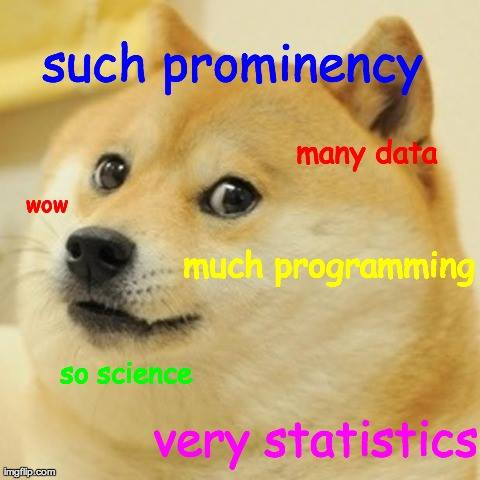
\includegraphics[width=8cm]{images/data_meme.jpg}
\caption{Placeholder}
\end{figure}
      
      
\subsection{Efficiency}[]
Number of evaluations to reach the same fitness
\begin{figure}[H]
\centering
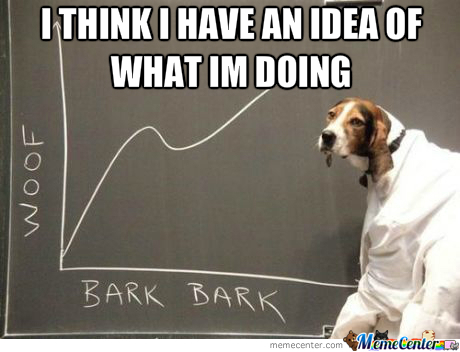
\includegraphics[width=8cm]{images/data_meme2.jpg}
\caption{Placeholder}
\end{figure}

\section{Future work}

In the second part of this internship, I will keep developing NeuroEvolution.jl (\textit{NE.jl}) and BERL jointly in order both to provide more stable and efficient tools, and to use them as a platform to design, implement and benchmark new algorithms. 

In this regard, the following points are currently forecast to be essential components of my work in the next months:
\begin{itemize}
    \item Adaptation of NeuroEvolution.jl and BERL.jl to Cambrian v0.2, which redefines the structure for a more robust and modular implementation
    \item Development of a CMA-ES-optimized neural network in NE.jl for weight-only evolution
    \item Study of alternative indirect encoding algorithms, e.g. Artificial Gene Regulatory Networks \cite{GRN}
    \item Introduction of other evolutionary algorithmic mechanisms such as coevolution or Quality-Diversity in the NEAT structure.
\end{itemize}

%%% Local Variables: 
%%% mode: latex
%%% TeX-master: "isae-report-template"
%%% End: 